\documentclass{article}
\usepackage[utf8]{inputenc}
\usepackage{enumerate}
\usepackage{enumitem}
\usepackage{float}
\usepackage{graphicx}
\usepackage{multirow, array}
\usepackage[spanish,activeacute]{babel}


\title{Práctica 2: Gestión de una Web de cine}
\author{Rafael Nogales Vaquero
\\Lothar Soto Palma
\\Elena Toro Pérez
\\Jose Ramón Trillo Vilchez}
\date{\today}

\begin{document}
\maketitle

\section{Driagramas de Conceptos}
	\subsection*{Gestión de usuarios}


	%Rafa Nogales
	\subsection*{Gestión de películas}
	\textbf{Problema:} Los \textbf{administradores} necesitan mantener un orden en las \textbf{películas} del sistema.
	 Tan solo los \textbf{usuarios VIP} podrán añadir películas.\\
	\textbf{Conceptos:} Administrador, Usuario VIP, Solicitudes de añadir Películas, Películas.\\
	\textbf{	Relaciones:}
		\begin{itemize}
			\item Los administradores añaden distribuciones de peliculas.
			\item Todos los usuarios (incluídos los administradores) consultan películas.
			\item Los administradores añaden estrenos de películas.
			\item Los administradores añaden premios de películas.
			\item Los administradores añaden trailers de películas.
			\item Los VIP pueden añadir películas y los administradores aceptar o denegar las solicitudes.		
		\end{itemize}
	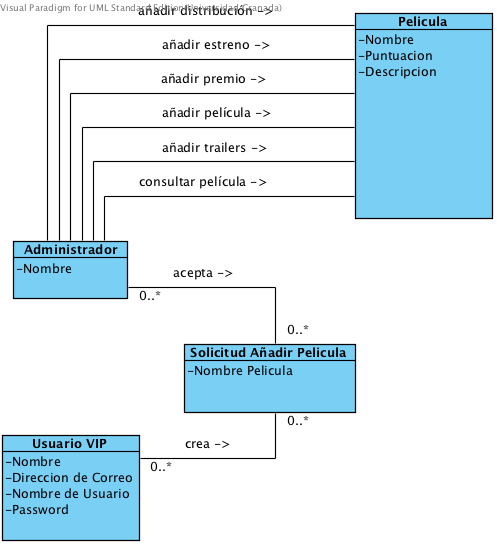
\includegraphics[width=0.7\linewidth]{./C-GestionDePeliculas}
	
	
	%Rafa Nogales
	\subsection*{Gestión de cartelera}
	\textbf{Problema:} Los \textbf{administradores} necesitan administrar los \textbf{cines} del sistema para saber en que horarios se proyectan 
	las \textbf{películas} en cada cine (\textbf{Programación}).
	\textbf{Conceptos:} Administrador, Cine, Programación, Películas.\\
	\textbf{	Relaciones:}
		\begin{itemize}
			\item Los administradores consultan la programación de las películas.
			\item Los administradores modifican la programación de las películas.
			\item Los administradores dan de alta las programaciones de las películas.
			\item Los administradores dan de alta cines.
			\item Los administradores dan de baja cines.
		\end{itemize}
	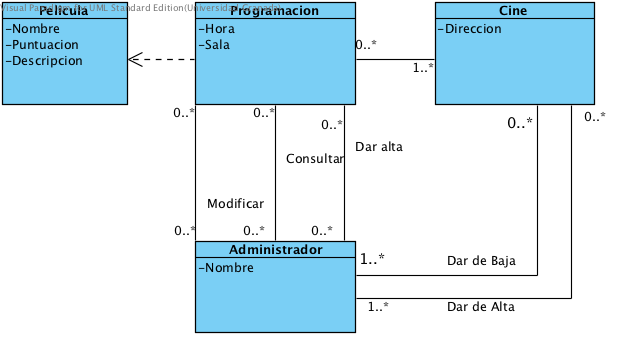
\includegraphics[width=0.7\linewidth]{./C-Cartelera}
	
	
	\subsection*{Gestión de Perfil}



	%Lothar Soto
	\subsection*{Gestión de películas por usuarios}
	\textbf{Problema:} Los \textbf{usuarios} podrán buscar \textbf{películas} en el sistema además de consultar la \textbf{cartelera} de \textbf{Cines}, solo si están \textbf{registrados} podrán puntuarla y tan solo los \textbf{usuarios VIP} podrán añadir y criticar películas.\\
	\textbf{Conceptos:} Usuario, Usuario registrado, Usuario VIP, Cines, Películas, Cartelera.\\
\textbf{	Relaciones:}
		\begin{itemize}
			\item Un cine tiene una cartelera.
			\item Todos los usuarios buscan películas.
			\item Todos los usuarios consultan la cartelera.
			\item Los registrados y los VIP pueden puntuar las películas.
			\item Los VIP pueden criticar y añadir películas.		
		\end{itemize}
			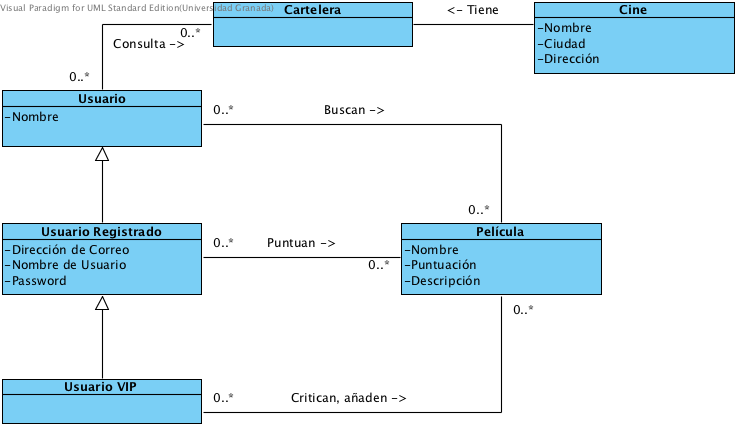
\includegraphics[width=1\linewidth]{./C-PeliculasUsuarios}
	
	%Lothar Soto	
	\subsection*{Gestión de comunidades}
	\textbf{Problema:} Un \textbf{usuario registrado} se va a encargar de crear \textbf{comunidades} y consultarlas. Los \textbf{usuarios} pueden pedir ser \textbf{miembro} de una \textbf{comunidad}, y si son \textbf{dueños} de una de ellas admitir otros \textbf{usuarios} en ellas. Por último pueden listar \textbf{películas} criticadas por una \textbf{comunidad} o anádidas por la misma.\\
	\textbf{Conceptos:} Usuario registrado, Comunidades, Miembro, Dueño.
	\textbf{Relaciones:}
		\begin{itemize}
			\item Los usuarios crean comunidades.
			\item Los usuarios consultan comunidades.
			\item Los usuarios son miembros de otras comunidades.
			\item Los usuarios son dueños de comunidades.
			\item Los usuarios pueden listar películas.
			\item Las películas pueden ser criticadas por la comunidad.
			\item Las películas pueden ser añadidas por la comunidad.
		\end{itemize}
		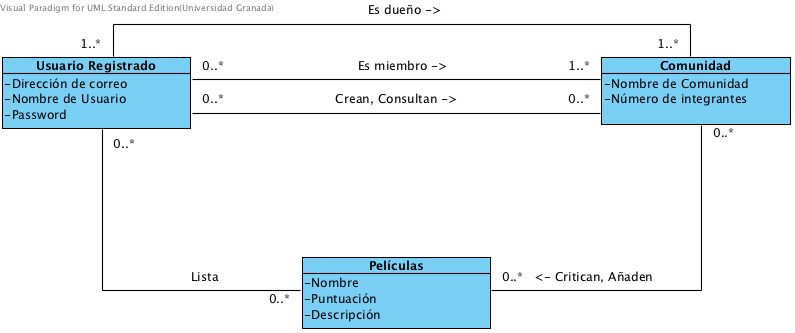
\includegraphics[width=1\linewidth]{./C-Comunidades}
		
\section{Driagramas de Secuencia}
	\subsection*{Gestión de usuarios}
	\subsection*{Gestión de películas}
	\subsection*{Gestión de cartelera}
	
			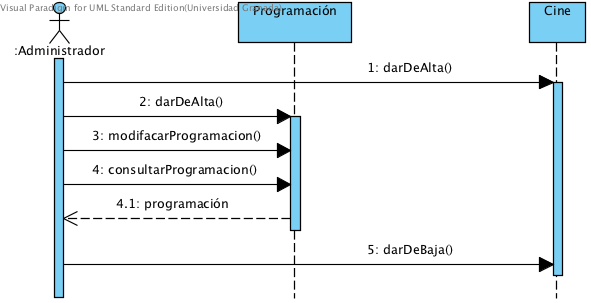
\includegraphics[width=1\linewidth]{./Sec-Cartelera}

	\subsection*{Gestión de Perfil}
	\subsection*{Gestión de películas por usuarios}
	\subsection*{Gestión de comunidades}
	\begin{enumerate}
		\item El usuario registrado ingresa en el sistema.
		\item Se dirige al apartado dedicado a la gestión de comunidades.
		\item Crea una comunidad aunque para ello debe rellenar un formulario.
		\item El Usuario que quiere ser miembro de una comunidad solicita entrar en ella.
		\item El Usuario dueño admite o no al anterior usuario.
		\item La comunidad añade películas y las critica.
		\item El Usuario es capaz de listar las películas criticadas y añadidas por la comunidad.
	\end{enumerate}
		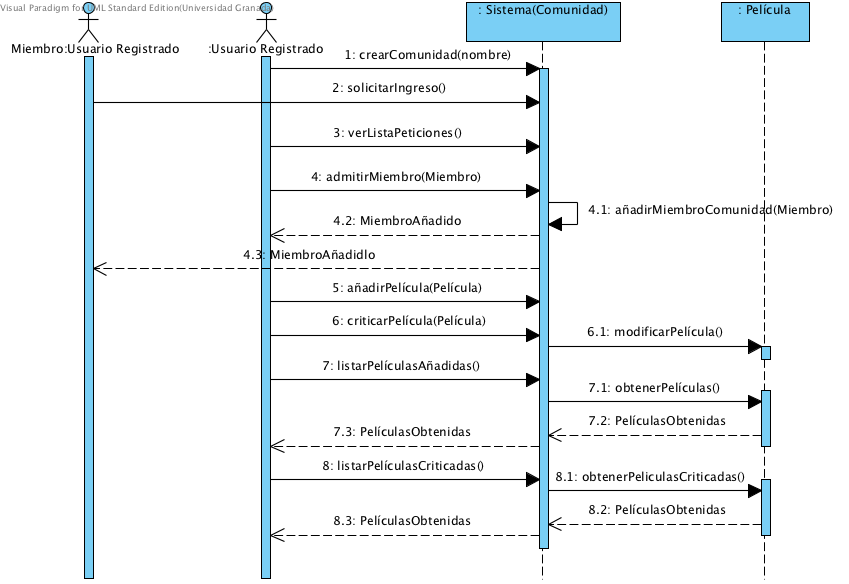
\includegraphics[width=1\linewidth]{./S-Comunidades}
\end{document}
